\documentclass{isprs}
\usepackage{setspace}
\usepackage{geometry}
\usepackage{epstopdf}
\usepackage[labelsep=period]{caption}
\usepackage{subcaption}
\usepackage[british]{babel}
\usepackage[hang]{footmisc}
\def\footnotemargin{1em}
\usepackage{textcomp}
\usepackage{amsmath}
\usepackage{booktabs}
\usepackage{url}
\usepackage{pdflscape}

\usepackage{hyperref}

\graphicspath{{plots/}}

% --------------------------------------------------------------------

\geometry{a4paper, top=25mm, left=20mm, right=20mm, bottom=25mm, headsep=10mm, footskip=12mm}

\captionsetup{justification=centering,font=normal}
\captionsetup[figure]{font=small}
\captionsetup[table]{font=small}

% --- float placement: many full-width figures/tables in two columns ---
\setcounter{topnumber}{3}
\setcounter{dbltopnumber}{3}
\setcounter{totalnumber}{5}
\renewcommand{\topfraction}{0.92}
\renewcommand{\dbltopfraction}{0.92}
\renewcommand{\textfraction}{0.06}
\renewcommand{\floatpagefraction}{0.7}
\renewcommand{\dblfloatpagefraction}{0.7}

% --- helper macros ---
\newcommand{\dg}{\textdegree}
\newcommand{\degC}{\textdegree C}
\newcommand{\tabbr}[1]{\texttt{#1}}
\newcommand{\kaBP}{ka\,BP}
\setlength{\emergencystretch}{3em}

\begin{document}

\title{A harmonised point-extraction and comparison tool for heterogeneous paleoclimate datasets}

\address{
	\begin{tabular}{ll}
	\textbf{Author:}	 & Levin Damian Antonin Giersch\\
	\textbf{Student ID:} & 0515040\\
	\textbf{E-Mail:}     & l.giersch@campus.tu-berlin.de\\
	\textbf{Faculty:}    & Faculty VI - Planning Building Environment\\
	\textbf{Program:}    & Geodesy and Geoinformation Science, M.Sc.\\
	\textbf{Lecturer:}   & Prof. Dr.-Ing. Martin Kada\\
	\textbf{Date:}       & \today\\
	\end{tabular}
}


\keywords{Paleoclimate, Data harmonisation, Paleoclimate datasets, Temperature comparison, Air temperature, Ground temperature, TraCE-21k, CHELSA-TraCE21k-centennial, PalMod2, Beyer2020}

\abstract{
Transient paleoclimate simulations and reconstructions are indispensable for understanding how the Earth system responds to forcing, yet they are distributed in mutually incompatible formats. Each archive uses a different time origin and unit, a different spatial grid and longitude convention, a different temperature variable, and a different temporal and spatial resolution. This project develops a small, reproducible Python toolchain that downloads four widely used temperature archives covering the last deglaciation, one of them the full last glacial cycle, namely TraCE-21k, CHELSA-TraCE21k-centennial, Beyer2020 and PalMod2. It harmonises their time axes onto a common kiloyears-before-present (\kaBP) scale, reconciles their longitude conventions and resolves each grid to the cell nearest a requested point, converts all temperatures to degrees Celsius, and then extracts and compares temperature time series at an arbitrary point as well as globally through pairwise mean-difference heatmaps. Applied to an example location in northern Germany ($\approx 53.26\dg$\,N, $11.67\dg$\,E), the four archives agree on the first-order signal, a cold Last Glacial Maximum (LGM) followed by deglacial warming into the Holocene, but disagree on absolute temperature by several degrees. The global comparison heatmaps show the largest systematic divergences at high northern latitudes and in mountain regions. The report documents the datasets, the acquisition and pre-processing pipeline, the harmonisation methods and the results, and discusses why these archives are difficult to compare and what the comparison reveals.
}

\maketitle

\pagestyle{plain}

\sloppy

%-------------------------------------------------------------

\section{Introduction}

\subsection{Why paleoclimate models matter}
The longest instrumental temperature records in Germany span about 320 years \cite{dwd_temp}, far too short to characterise the full range of natural climate variability or to observe the slow processes (ice-sheet growth and decay, ocean-circulation reorganisations, orbital forcing) that govern the climate system on millennial timescales. Numerical paleoclimate simulations and data-constrained reconstructions extend our knowledge of temperature across the last glacial cycle and beyond. They are useful for: reconstructing Earth's climate before direct measurements existed, understanding how the climate responds to forcings such as solar output, volcanic eruptions, Milankovi\'c cycles, greenhouse gases and changing ice sheets, testing and validating modern climate models against known past states, establishing the natural variability range of climate, separate from human influence, constraining climate sensitivity (the temperature change per CO\textsubscript{2} doubling) using the large glacial-interglacial signal and using past warm periods as analogues for near-future projections.

\subsection{Why intercompare models}
No single archive is ``correct''. Coupled general-circulation models (GCMs) such as those behind TraCE-21k and PalMod2 simulate the physics explicitly but at coarse resolution; statistical reconstructions and downscaling products such as Beyer2020 and CHELSA-TraCE21k-centennial achieve high spatial resolution by anchoring model output to present-day observations, at the cost of the assumptions built into the downscaling. Comparing them is therefore important: systematic differences reveal where the archives are robust and where they diverge, expose outliers and artefacts, and help target the processes or regions where the underlying models most need improvement. A comparison cannot say which archive is right, but it can say where and by how much they disagree.

\subsection{Aim and scope}
The aim of this project is a harmonised point-extraction and comparison tool for four heterogeneous paleoclimate temperature archives. Given a latitude and longitude, the tool extracts a near-surface air-temperature (and, where available, soil-temperature) time series from each archive, reconciles their incompatible time axes, spatial grids and units, and produces (i) per-dataset inspection reports, (ii) a temperature time-series overlay at the requested point, (iii) a side-by-side summary of temporal coverage and the grid cell each archive returns near the point, and (iv) global pairwise mean-difference heatmaps. The workflow is organised as three Jupyter notebooks: a downloader, a pre-processor, and the comparison and exploration notebook \cite{giersch2026_paleoclimate_model_comparison}.

\subsection{Study area and example point}
All point-based results below are shown for a single terrestrial location in northern Germany ($\approx 53.26\dg$\,N, $11.67\dg$\,E, south-western Mecklenburg, near the lower Elbe). The location is used purely as a worked example; the tool accepts any coordinate. It is mid-latitude, continental and ice-free throughout the studied interval, which makes it a convenient case for examining how the four archives represent the deglacial warming at one place.

\section{The data}
Four archives were selected to span the trade-off between temporal resolution, spatial resolution and time coverage. Two are raw transient GCM simulations (TraCE-21k, PalMod2); two are high-resolution, observation-anchored products (Beyer2020, CHELSA-TraCE21k-centennial). Table~\ref{tab:overview} summarises them. All are downloaded via the \tabbr{data\_downloader} notebook; the total download is on the order of 1\,TB, dominated by the $\sim$1\,km CHELSA-TraCE21k-centennial GeoTIFFs.

\begin{table*}[t]
\centering
\small
\begin{tabular}{lllllll}
\toprule
Dataset           			& Type                        & Variables   & Coverage     & Time step  & Native res.           	& Unit \\
\midrule
TraCE-21k         			& Coupled GCM (CCSM3)         & TSA, TSOI   & 22--0 \kaBP  & decadal    & T31 ($\sim$3.71/3.75\dg)   	& K \\
PalMod2           			& Coupled GCM (MPI-ESM1.2-CR) & tas, tsl    & 25--0 \kaBP  & annual     & T31 ($\sim$3.71/3.75\dg)   	& K \\
Beyer2020/21 (v4)			& Downscaled reconstruction   & temperature & 120--0 \kaBP & 2/1 kyr    & 0.5\dg{}              	& \degC \\
CHELSA-TraCE21k-centennial  & Downscaled product          & tasmean     & 22--0 \kaBP  & centennial & $\sim$1\,km (30\,arcsec) 	& K \\
\bottomrule
\end{tabular}
\caption{Overview of the four temperature archives.}
\label{tab:overview}
\end{table*}

\subsection{TraCE-21k}
TraCE-21k (the ``Simulation of the Transient Climate of the Last 21,000 Years'', here the TraCE-21k Main Land Decadal Average product) is a fully coupled, non-accelerated atmosphere-ocean-sea-ice-land-surface transient simulation produced with the Community Climate System Model version 3 (CCSM3), its land component being the Community Land Model 2 (CLM2). It integrates forward from the LGM under transient orbital, greenhouse-gas, ice-sheet and meltwater forcing and is one of the foundational transient deglaciation experiments. The atmosphere and land grid is T31\_gx3 ($\sim$3.75\dg, 96 longitudes $\times$ 48 latitudes). The used variables are TSA (2\,m air temperature) and TSOI (soil temperature on 10 layers), delivered as two NetCDF files totalling $\approx$449\,MB ($\approx$41\,MB for TSA, $\approx$406\,MB for TSOI); time runs from 22 \kaBP{} to present as decadal averages (2204 steps). Access is via the NCAR GDEX archive (dataset d651050); variable codes are listed in the TraCE-21k variable table. Source: \cite{trace21k_data} \cite{trace_vars}.

\subsection{CHELSA-TraCE21k-centennial}
CHELSA-TraCE21k-centennial is a high-resolution ($\sim$1\,km) downscaled product of transient temperature and precipitation since the LGM, generated with the CHELSA-TraCE21k downscaling model \cite{chelsa_trace21k_paper,chelsa_trace21k_data}. The centennial variant used here provides monthly climatologies at 100-year time steps, at a native resolution of $\sim$1\,km (30\,arcsec, $\approx 0.0083\dg$), globally. The used variables are \tabbr{tasmax} and \tabbr{tasmin}; the mean air temperature is derived as $\mathrm{tasmean} = (\mathrm{tasmax}+\mathrm{tasmin})/2$ in the data\_processor notebook \cite{giersch2026_paleoclimate_model_comparison}. The data arrive as GeoTIFF (one raster per month, per time index, per variable) and must be converted to NetCDF; coverage is 22 \kaBP{} to present in centennial steps (221 time steps). The $\sim$1\,km tiffs dominate the download. Source: \cite{chelsa_trace21k_paper}; data \cite{chelsa_trace21k_data}.

\subsection{Beyer2020}
Beyer2020 (version-4 / ``2021'' update is used) reconstructs high-resolution terrestrial climate, bioclimate and vegetation for the last 120,000 years, produced at the Department of Zoology, University of Cambridge \cite{beyer2020_paper,beyer2021_addendum}. It was built by a delta-method downscaling and bias-correction procedure that combines medium-resolution transient HadCM3 simulations with high-resolution HadAM3H time-slice snapshots and present-day observational climatology, bridging the gap between high-temporal-resolution but coarse simulations and high-spatial-resolution but snapshot-only datasets. The used variable is \tabbr{temperature} (monthly mean, \degC), delivered as a single bundled NetCDF on a 0.5\dg{} equirectangular grid ($720\times300$, $\sim$55\,km at the equator), global terrestrial only (latitudes $\approx 60\dg$\,S to $90\dg$\,N). Coverage is 120 \kaBP{} to pre-industrial in 72 snapshots, with 2000-year steps from 120--22 \kaBP{} and 1000-year steps from 22--0 \kaBP. The v4 release adds global monthly NPP relative to v3, documented in the 2021 addendum. Source: \cite{beyer2020_paper}, \cite{beyer2021_addendum} and \cite{beyer2021_data_4}.

\subsection{PalMod2}
PalMod2 here denotes the MPI-M MPI-ESM1.2-CR Transient Simulations of the Last Deglaciation with prescribed ice sheets from GLAC-1D reconstructions (r1i1p1f1), produced at the Max Planck Institute for Meteorology and DKRZ \cite{palmod2_data}. It is a fully coupled transient simulation with MPI-ESM1.2 in coarse resolution (MPI-ESM1.2-CR): the ECHAM6.3 spectral atmosphere at T31 ($96\times48$, 31 levels), the JSBACH3.20 land surface, and the MPIOM1.63 ocean ($\sim$300\,km), with realistic time-evolving ice-sheet, topography and land-sea-mask forcing from GLAC-1D. The used variables are \tabbr{tas} (near-surface, usually 2\,m, air temperature; \texttt{PMMXMCRTDGr111\allowbreak Amtasgn30201}) and \tabbr{tsl} (soil temperature by layer; \texttt{PMMXMCRTDGr111\allowbreak Lmtslgn30201}), both monthly, in K; the native time coverage is the last $\sim$25\,kyr. Access is through the WDCC archive at DKRZ, downloaded via the \tabbr{jblob} client after registration \cite{wdcc_jblob}; model output is licensed CC-BY-SA 4.0. Source: \cite{palmod2_data}.

\subsection{Data acquisition}
Each archive uses a different access mechanism (Table~\ref{tab:acq}). PalMod2 is the only one requiring authentication: a WDCC account must be created (registration may take several days) and the \tabbr{jblob} client obtained from the WDCC site. The downloader skips files that already exist, so it is safe to re-run.

\begin{table*}[t]
\centering
\small
\begin{tabular}{lll}
\toprule
Dataset          			& Host                  & Mechanism \\
\midrule
TraCE-21k        			& NCAR GDEX (d651050)   & Direct HTTP; filtered to TSA/TSOI. \\
CHELSA-TraCE21k-centennial  & EnviDat / SwitchCH S3 & Parallel download (32 threads), atomic \tabbr{.part} rename. \\
Beyer2020   				& figshare API          & Query API for version 4 of article 12293345. \\
PalMod2          			& WDCC / DKRZ           & \tabbr{jblob} client, login automated via \tabbr{pexpect}. \\
\bottomrule
\end{tabular}
\caption{Acquisition mechanism per dataset.}
\label{tab:acq}
\end{table*}

\section{Pre-processing}
Two of the four archives cannot be used as delivered. The \tabbr{data\_processor} notebook performs the necessary conversions on CHELSA-TraCE21k-centennial and PalMod2. TraCE-21k and Beyer2020 are already analysis-ready NetCDF and are passed through unchanged.

\subsection{CHELSA-TraCE21k-centennial: GeoTIFF to centennial-mean NetCDF}
The CHELSA-TraCE21k-centennial product arrives as one GeoTIFF per month, per time index, per variable, named \tabbr{CHELSA\_TraCE21k\_<var>\_<MM>\_<TTT>\_V.1.0.tif}, where \tabbr{MM} is the month and \tabbr{TTT} a centennial time index. The data\_processor notebook first groups files by year: a regex extracts month and index, and the index is mapped to a calendar year by $\mathrm{year} = 1990 - (20 - \mathrm{TTT})\times100$, anchored at $\mathrm{TTT}=20 \rightarrow 1990$\,CE with 100-year steps. Thus index 0 maps to about year $-10$\,CE and index $-200$ to about $-20010$\,CE ($\approx 22$ \kaBP, near the LGM). This mapping is consistent with the file's \tabbr{frequency=centennial} metadata, the $\sim$21,000-year nominal coverage and the file count (221 steps $\times$ 100 years $\approx 22$\,kyr); the exact index-to-year table is not published by CHELSA-TraCE21k-centennial, so the mapping is a well-constrained reconstruction, flagged as such in the notebook. For each year the 12 monthly rasters are stacked and averaged to one (lat, lon) field; CHELSA-TraCE21k-centennial stores temperature as Kelvin $\times$ 10, so a factor of 0.1 is applied and the result cast back to \tabbr{float32}. All years are concatenated along a new time axis (one timestamp at 1~July of each year), tagged with CF-style metadata, and written as one gzip-compressed NetCDF per variable at the full native $\sim$1\,km resolution. Finally $\mathrm{tasmean} = (\mathrm{tasmin}+\mathrm{tasmax})/2$ is derived. \cite{giersch2026_paleoclimate_model_comparison}

Because the full-resolution inputs are very large (on the order of $\sim$100\,GB each), every step before the write is lazy: only a Dask task graph is built. Data are materialised chunk by chunk during \tabbr{to\_netcdf}, so peak memory is set by the chunk size ($4500\times2250\times4$ bytes $\approx 40$\,MB) times the number of workers, not by the full array. The \tabbr{astype("float32")} after each floating-point operation is deliberate: multiplying by a Python float upcasts to float64, and casting back keeps the data at 4 bytes per pixel.

\subsection{PalMod2: monthly to annual means and merge}
The PalMod2 \tabbr{tas} and \tabbr{tsl} variables are delivered as monthly NetCDF files (250 per variable). For each variable the processor applies \tabbr{cdo yearmean} to collapse the 12 monthly values of each file into annual means, then \tabbr{cdo mergetime} to concatenate all annual-mean files along the time axis. To keep CDO from ever seeing the space-containing project path, the commands run from within the extraction directory using relative filenames. The merged outputs have 25,000 annual time steps.

\section{Harmonisation}
The four archives cannot be compared until they share a common footing in variable, time, space and unit. This is the analytical core of the project, performed in the paleoclimate\_comparison notebook. \cite{giersch2026_paleoclimate_model_comparison}

\subsection{Variables}
The comparison restricts itself to near-surface air temperature (and, separately, soil temperature), the only quantities common to enough archives to be comparable. Even so the variables are not strictly identical (Table~\ref{tab:vars}): TraCE-21k \tabbr{TSA} and PalMod2 \tabbr{tas} are model 2\,m air temperatures; Beyer2020 \tabbr{temperature} is a downscaled, bias-corrected monthly mean; CHELSA-TraCE21k-centennial \tabbr{tasmean} is the mean of downscaled daily extremes. These are physically close but not interchangeable, a caveat carried into the results. For soil temperature, only PalMod2 and TraCE-21k provide a layered variable; the comparison keeps the topmost soil layer (for TraCE, \tabbr{levsoi}[0] $\approx 0.007$\,m).

\begin{table*}[t]
\centering
\small
\begin{tabular}{lllll}
\toprule
Dataset   					& Air var.    & Soil var.    & Unit  & Native averaging \\
\midrule
Beyer2020					& temperature & --           & \degC & monthly $\rightarrow$ annual \\
PalMod2						& tas         & tsl (layer)  & K     & monthly $\rightarrow$ annual \\
TraCE-21k 					& TSA         & TSOI (layer) & K     & decadal average \\
CHELSA-TraCE21k-centennial  & tasmean     & --           & K     & centennial clim. \\
\bottomrule
\end{tabular}
\caption{Temperature variables harmonised.}
\label{tab:vars}
\end{table*}

\subsection{Time}
Every archive encodes time differently (different origin, sign convention and unit), so a single function, \tabbr{time\_to\_ka\_bp}, centralises the translation to a common scale of kiloyears before present, with the past positive and the present at zero (Table~\ref{tab:time}). For the two ``days since'' archives the absolute reference date is irrelevant: only the elapsed time before the most recent sample matters, so the conversion anchors on \tabbr{vals.max()} and divides by $365250 = 1000\times365.25$ days ($=1$\,kyr in a proleptic-Gregorian calendar). The $\sim$0.5\,ka rounding this can introduce is invisible on a 0--125\,ka axis. After conversion the archives span 0--120\,\kaBP{} (Beyer2020), 0--25\,\kaBP{} (PalMod2) and 0--22\,\kaBP{} (TraCE-21k and CHELSA-TraCE21k-centennial). The temporal resolution also differs by three orders of magnitude (annual, decadal, centennial and 1--2\,kyr), which directly affects how much high-frequency variability each archive exposes.

\begin{table*}[t]
\centering
\small
\begin{tabular}{llll}
\toprule
Dataset						& \tabbr{units} attribute                       & Raw range             & Conversion \\
\midrule
Beyer2020					& \tabbr{years since present} (past negative)   & $[-120000,\,0]$       & $-\mathrm{vals}/1000$ \\
PalMod2						& \tabbr{days since 1-1-1} (forward to present) & $[181,\,9\,130\,878]$ & $(\max-\mathrm{vals})/365250$ \\
TraCE-21k					& \tabbr{ka BP} (stored negative)               & $[-22,\,0.03]$        & $-\mathrm{vals}$ \\
CHELSA-TraCE21k-centennial	& \tabbr{days since -20010-07-01} (forward)     & $[0,\,8\,035\,335]$   & $(\max-\mathrm{vals})/365250$ \\
\bottomrule
\end{tabular}
\caption{Time-axis conventions and conversion to \kaBP.}
\label{tab:time}
\end{table*}

\subsection{Space}
The archives sit on four grids (Table~\ref{tab:space}) and use two longitude conventions (0--360\dg{} and $-180$--180\dg). The tool detects latitude and longitude coordinates by name and, before any query, converts a requested negative longitude to 0--360\dg{} when the file demands it. The spatial-resolution mismatch is severe: a single PalMod2 or TraCE-21k cell ($\sim$3.7\dg) is roughly 250\,km $\times$ 410\,km at 53\dg\,N, whereas a CHELSA-TraCE21k-centennial pixel (0.0083\dg) is about 1\,km and a Beyer2020 cell (0.5\dg) about 55\,km. PalMod2 and TraCE-21k share the same T31 grid, so their cells coincide exactly.

\begin{table*}[t]
\centering
\small
\begin{tabular}{llllll}
\toprule
Dataset   					& Grid                    & Lat range                   & Lon range                     & Convention  & Res. \\
\midrule
Beyer2020					& $720\times300$          & $-59.75\dg \ldots 89.75\dg$ & $-179.75\dg \ldots 179.75\dg$ & $-180$--180 & 0.5\dg \\
PalMod2						& $96\times48$ (Gaussian) & $-87.16\dg \ldots 87.16\dg$ & $0\dg \ldots 356.25\dg$       & 0--360      & $\sim$3.71/3.75\dg \\
TraCE-21k					& $96\times48$            & $-87.16\dg \ldots 87.16\dg$ & $0\dg \ldots 356.25\dg$       & 0--360      & $\sim$3.71/3.75\dg \\
CHELSA-TraCE21k-centennial	& global $\sim$1\,km      & global                      & global                        & $-180$--180 & 0.0083\dg \\
\bottomrule
\end{tabular}
\caption{Spatial grids (native resolutions).}
\label{tab:space}
\end{table*}

\subsection{Units}
PalMod2, TraCE-21k and CHELSA-TraCE21k-centennial store temperature in kelvin; Beyer2020 in degrees Celsius. All extracted series are converted to \degC{} (subtracting 273.15\,K where required) before plotting or differencing, so every figure is in a single, intuitive unit.

\section{Point extraction}
\label{sec:extraction}
The function \tabbr{extract\_temperature\_at\_point} returns a 1-D temperature series (in \degC, on the \kaBP{} axis) for one file at a requested coordinate. It (i) opens the file without decoding times; (ii) selects the nearest grid cell with \tabbr{xarray.sel(method="nearest")} after translating the requested longitude into the file's convention, a plain nearest-neighbour lookup with no interpolation, recording the actual cell-centre coordinates; (iii) collapses extra dimensions (keeps the topmost soil layer if a depth dimension is present, averages a month dimension to an annual mean); and (iv) converts kelvin to \degC{} when needed. The same logic underlies the summary plots, so the text report, the time-series overlay and the grid-cell map cannot disagree about which cell was used.

The extraction is not restricted to a single location. It is driven from a \tabbr{poi} dictionary that maps a label to a (latitude, longitude) pair, over whose entries the notebook iterates, so an arbitrary set of points is processed in one run and the extracted series are retained per location. The helper \tabbr{grid\_cell\_centers} returns every cell centre of a given file in the same dictionary format, optionally restricted to a bounding box by \tabbr{filter\_europe}, so the same machinery can also be pointed at a whole grid rather than at hand-picked coordinates. All point-based results shown in Section~\ref{sec:results} use a single entry, the example location in northern Germany.

\section{Inter-model comparison method}
\label{sec:comparison}
Beyond the single-point series, the tool produces global pairwise mean-difference heatmaps. For a pair of archives $A$ and $B$: (1) a \emph{shared time window} is computed from the two time axes (their overlap), read cheaply from the time coordinate alone, so both means cover the same interval; (2) a \emph{common sampling grid} is used, namely every cell centre of the T31 grid shared by PalMod2 and TraCE-21k ($96\times48 = 4608$ points), and for each archive the temperature at each point is read with a vectorised nearest-neighbour index, averaged over the shared window and converted to \degC; (3) the difference $A-B$ is drawn on a PlateCarree world map with the diverging PRGn colormap and a TwoSlopeNorm centred at zero (green $=A$ warmer, purple $=A$ colder), and cells where either archive has no data (for example ocean cells for the terrestrial Beyer2020 and CHELSA-TraCE21k-centennial archives) remain blank.

Because the shared sampling grid is the \emph{coarse} T31 grid, the high-resolution archives (Beyer2020 at 0.5\dg, CHELSA-TraCE21k-centennial at $\sim$1\,km) are effectively sub-sampled, one representative pixel per $\sim$3.7\dg{} cell, rather than area-averaged into the coarse cell. This keeps the heatmaps fast and memory-bounded but means they compare \emph{point samples}, not area means (see Section~\ref{sec:caveats}). The point-extraction time-series plots, by contrast, use each archive at its native resolution; in particular CHELSA-TraCE21k-centennial is read at its full $\sim$1\,km grid, so the returned CHELSA-TraCE21k-centennial cell matches the requested point to within one $\sim$1\,km pixel ($\approx 0.0083\dg$).

\section{Results}
\label{sec:results}

\subsection{Air-temperature time series at the example point}
\begin{figure*}[t]
\centering
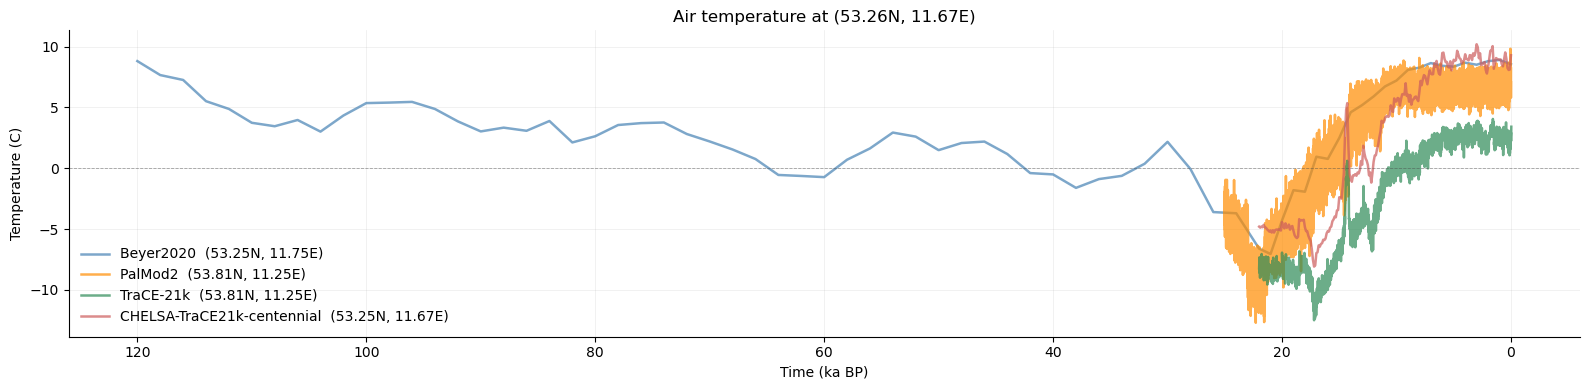
\includegraphics[width=0.98\textwidth]{ts_air_all.png}
\caption{Near-surface air-temperature time series at $\approx 53.26\dg$\,N, $11.67\dg$\,E (\kaBP{} on the $x$-axis, \degC{} on the $y$-axis), for all four archives. Each legend entry reports the grid-cell centre returned by the nearest-neighbour lookup.}
\label{fig:ts_air}
\end{figure*}

Figure~\ref{fig:ts_air} shows that Beyer2020 (blue), the only archive spanning the full 120\,kyr, reproduces the expected glacial-interglacial structure: a warm last interglacial ($\sim$9\,\degC{} around 120\,ka), a long oscillating cooling, a cold interval around the LGM (dropping to $\approx -4$\,\degC{} near 20--25\,ka), and deglacial warming to $\sim$8--9\,\degC{} in the Holocene; its 1--2\,kyr step makes the curve smooth. PalMod2 (orange) and TraCE-21k (green) begin near the LGM and, at their native annual and decadal resolution, expose large high-frequency variability. CHELSA-TraCE21k-centennial (red) tracks the deglacial warming at centennial resolution and reaches the warmest late-Holocene values here. In the overlapping window the four agree on the shape of the signal but disagree on absolute temperature by several degrees; most conspicuously, TraCE-21k settles to a noticeably cooler Holocene plateau ($\sim$3\,\degC) than the other three ($\sim$7--9\,\degC), an offset of order 4--5\,\degC{} that recurs in the heatmaps below. Part of the offset is a scale artefact: the coarse GCMs return a $\sim$3.7\dg{} cell centred at $\sim$53.8\dg\,N, 11.25\dg\,E, which averages a large, partly maritime region, whereas Beyer2020 and CHELSA-TraCE21k-centennial resolve the land point itself (Fig.~\ref{fig:cov_air}). 

\subsection{Soil-temperature time series at the example point}
\begin{figure*}[t]
\centering
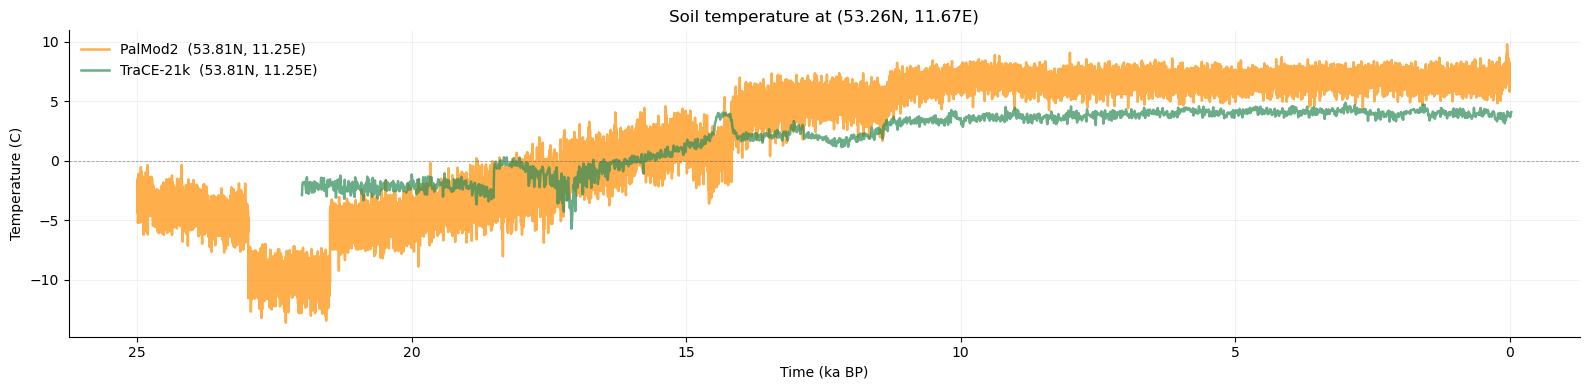
\includegraphics[width=0.98\textwidth]{ts_soil_palmod2_trace21k.png}
\caption{Top-layer soil-temperature time series at the example point for PalMod2 and TraCE-21k (the only two archives with a soil variable).}
\label{fig:ts_soil}
\end{figure*}

The soil comparison (Fig.~\ref{fig:ts_soil}) mirrors the air signal: both archives warm through the deglaciation, with PalMod2 again showing much larger interannual spread and abrupt multi-millennial steps and a warmer Holocene soil temperature ($\sim$6--8\,\degC) than TraCE-21k ($\sim$4\,\degC, smoother). The systematic warm offset of PalMod2 relative to TraCE-21k echoes the air-temperature relationship and the high-latitude divergence seen globally.

\subsection{Temporal coverage and the returned grid cells}
These summary panels (Figs.~\ref{fig:cov_air}--\ref{fig:cov_soil}) make the harmonisation challenge concrete. The coverage panel shows the three-order-of-magnitude spread in time step (Beyer $\Delta t \approx 2000$\,yr, $n=72$; PalMod2 $\approx 1$\,yr, $n=25000$; TraCE-21k $\approx 10$\,yr, $n=2204$; CHELSA-TraCE21k-centennial $\approx 100$\,yr, $n=221$) and the very different coverage windows. The grid-cell panel shows the spatial-scale mismatch directly: the PalMod2 and TraCE-21k cells ($\sim$3.7\dg, overlapping exactly) form one large rectangle spanning much of northern Germany and the western Baltic, the Beyer2020 cell (0.5\dg) is small, and the CHELSA-TraCE21k-centennial cell (0.0083\dg) is effectively a point. The coarse cells visibly straddle land and sea, which biases their temperature relative to the high-resolution land-only archives.

\begin{figure*}[t]
\centering
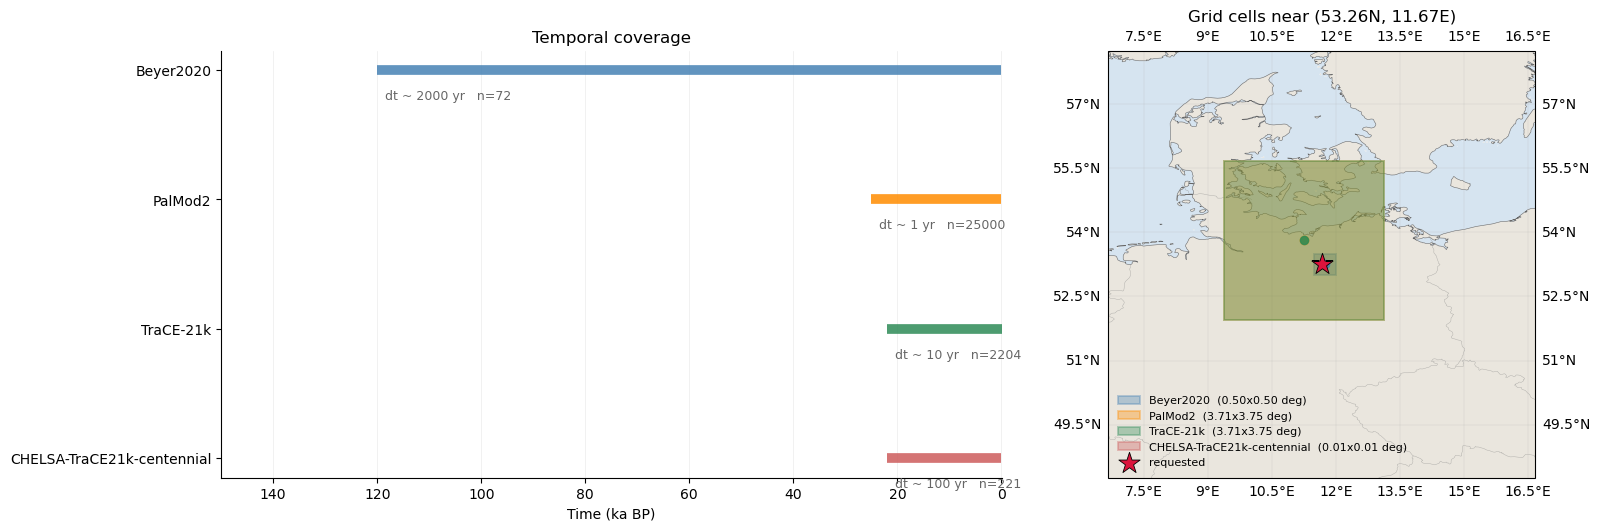
\includegraphics[width=0.98\textwidth]{coverage_air_all.png}
\caption{Air archives. Left: temporal coverage (bar length $=$ covered interval; annotation $=$ time step and number of samples). Right: the grid cell each archive returns near the example point, drawn at its true size in degrees, over a regional basemap.}
\label{fig:cov_air}
\end{figure*}

\begin{figure*}[t]
\centering
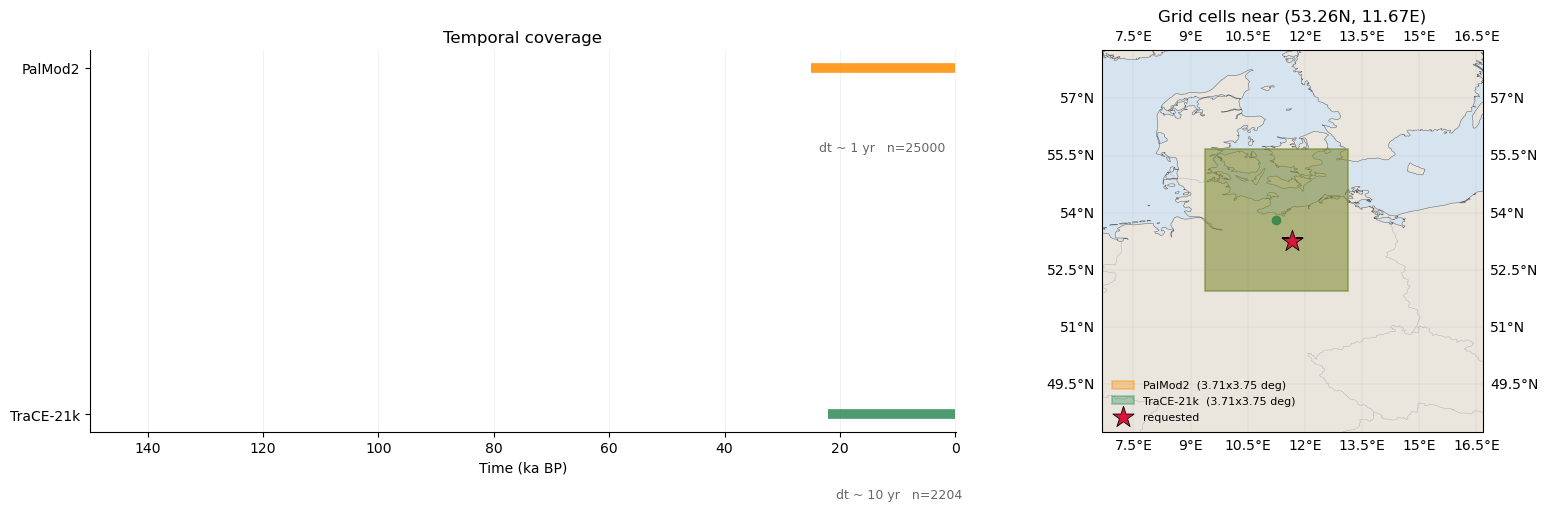
\includegraphics[width=0.98\textwidth]{coverage_soil_palmod2_trace21k.png}
\caption{As Fig.~\ref{fig:cov_air}, for the two soil archives (PalMod2, TraCE-21k).}
\label{fig:cov_soil}
\end{figure*}

\subsection{Global pairwise difference heatmaps}
The difference maps are computed on the shared $96\times48 = 4608$-cell T31 grid described in Section~\ref{sec:comparison}.

\paragraph{Soil temperature.} PalMod2 is markedly warmer than TraCE-21k across the high northern latitudes (northern Eurasia and North America, locally by $\sim$10--15\,\degC), with smaller patches where PalMod2 is cooler (Fig.~\ref{fig:diff_soil}). The dominant signal is a systematic high-latitude divergence between the two GCMs. TraCE-21k appears to be warmer in high mountain ranges such as the Himalayas and the Andes.

\begin{figure*}[t]
\centering
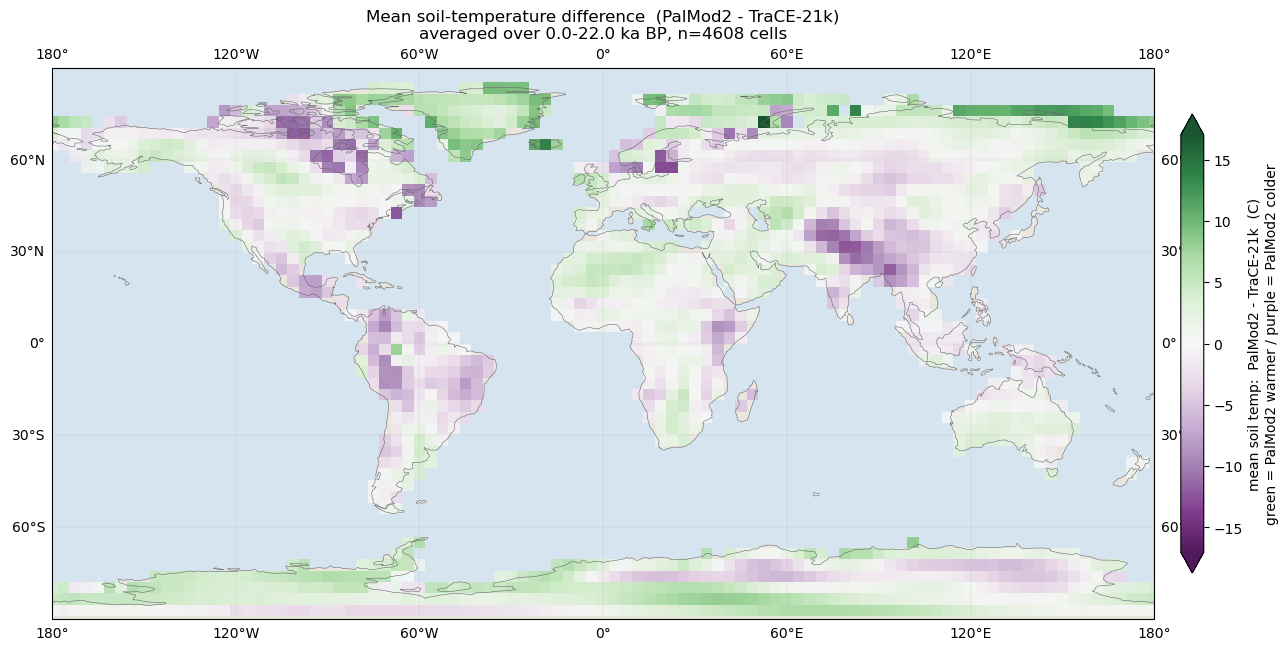
\includegraphics[width=0.72\textwidth]{diff_soil_palmod2_trace21k.png}
\caption{Mean top-layer soil-temperature difference, PalMod2 $-$ TraCE-21k, averaged over the shared 0--22\,\kaBP{} window (green $=$ PalMod2 warmer, purple $=$ PalMod2 colder).}
\label{fig:diff_soil}
\end{figure*}

\paragraph{Air temperature, all six pairs.} The four air archives yield six pairwise comparisons (Figs.~\ref{fig:diff_air_beyer_palmod2}--\ref{fig:diff_air_trace21k_chelsa}), each averaged over the shared window noted in the caption. The maps show that Beyer2020 is generally warmer than PalMod2 across the tropics, mid-latitudes and mountain ranges but markedly colder over the high-northern continents (Fig.~\ref{fig:diff_air_beyer_palmod2}); Beyer2020 is warmer than TraCE-21k almost everywhere, most strongly over northern Eurasia (Fig.~\ref{fig:diff_air_beyer_trace21k}); Beyer2020 and CHELSA-TraCE21k-centennial, the two observation-anchored products, are the most similar pair, with only faint differences, except for high northern latitudes where CHELSA-TraCE21k-centennial is warmer in most cells (Fig.~\ref{fig:diff_air_beyer_chelsa}); the two GCMs differ strongly and coherently, PalMod2 is much warmer than TraCE-21k at high northern latitudes and cooler over the Southern Ocean margin and in mountain ranges (Fig.~\ref{fig:diff_air_palmod2_trace21k}); PalMod2 $-$ CHELSA-TraCE21k-centennial is moderate and patchy (Fig.~\ref{fig:diff_air_palmod2_chelsa}); and TraCE-21k is colder than CHELSA-TraCE21k-centennial across most land, again strongest in the high north (Fig.~\ref{fig:diff_air_trace21k_chelsa}).

\begin{figure*}[t]
\centering
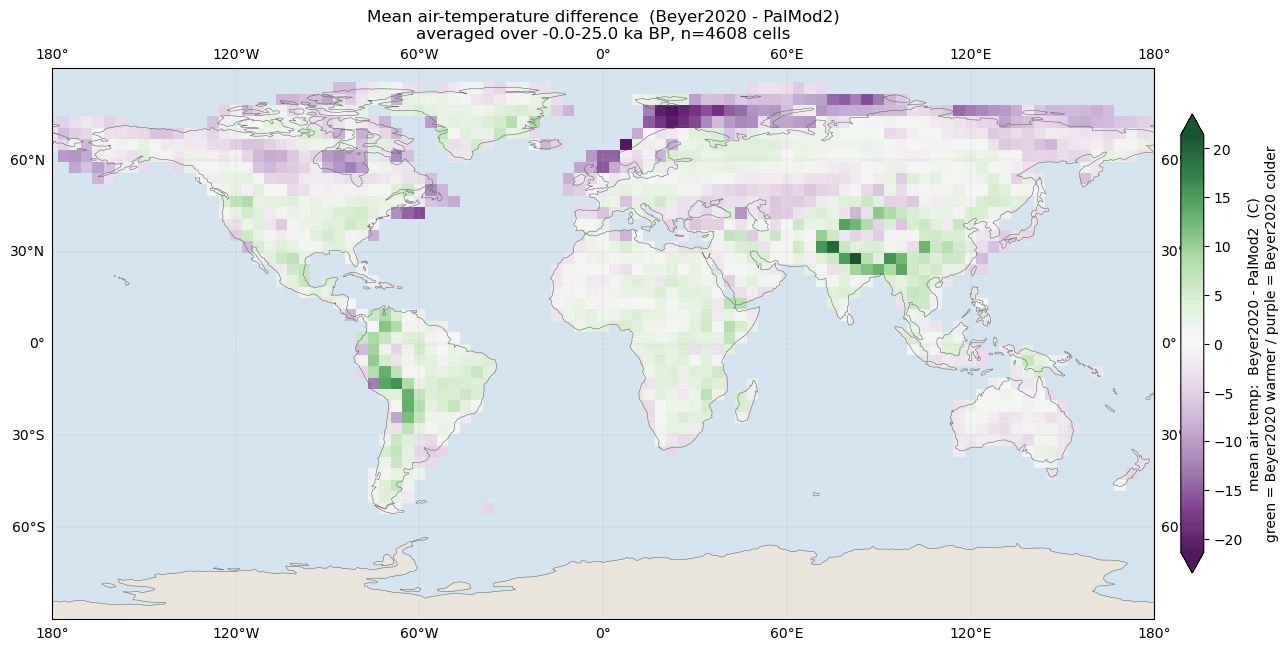
\includegraphics[width=0.72\textwidth]{diff_air_beyer2020_palmod2.png}
\caption{Mean air-temperature difference, Beyer2020 $-$ PalMod2 (0--25\,ka), sampled at the T31 grid and averaged over the pair's shared time window (green $=$ first archive warmer, purple $=$ colder).}
\label{fig:diff_air_beyer_palmod2}
\end{figure*}

\begin{figure*}[t]
\centering
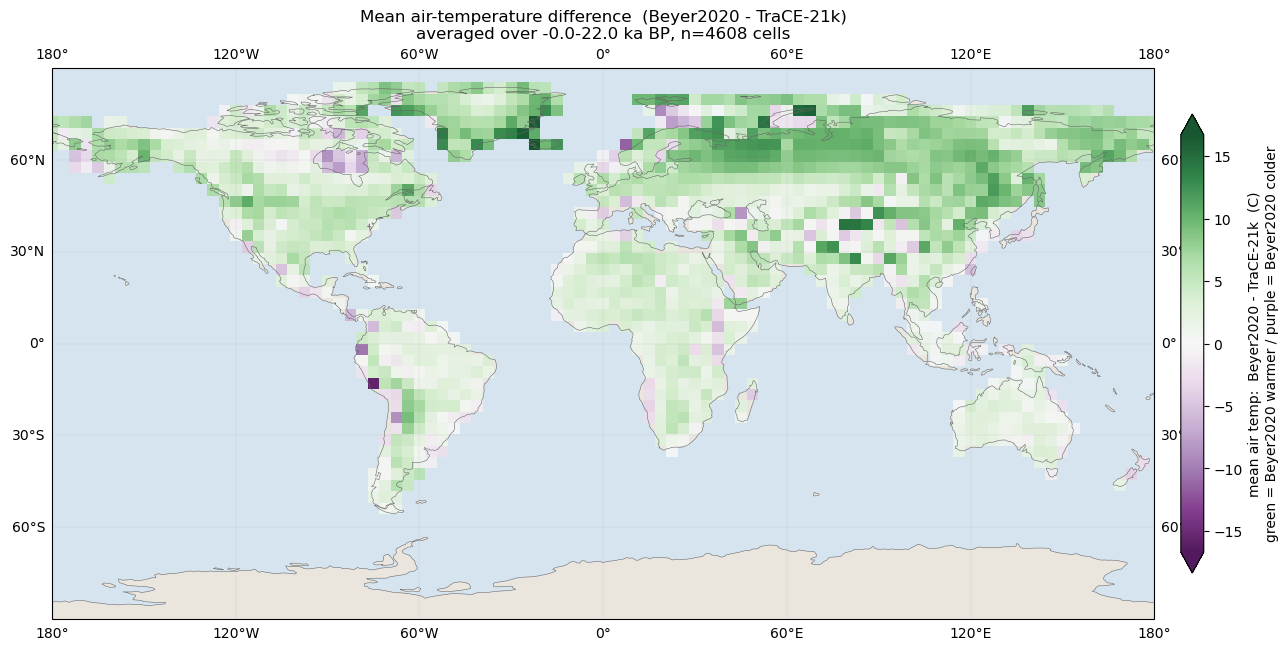
\includegraphics[width=0.72\textwidth]{diff_air_beyer2020_trace21k.png}
\caption{Mean air-temperature difference, Beyer2020 $-$ TraCE-21k (0--22\,ka), sampled at the T31 grid and averaged over the pair's shared time window (green $=$ first archive warmer, purple $=$ colder).}
\label{fig:diff_air_beyer_trace21k}
\end{figure*}

\begin{figure*}[t]
\centering
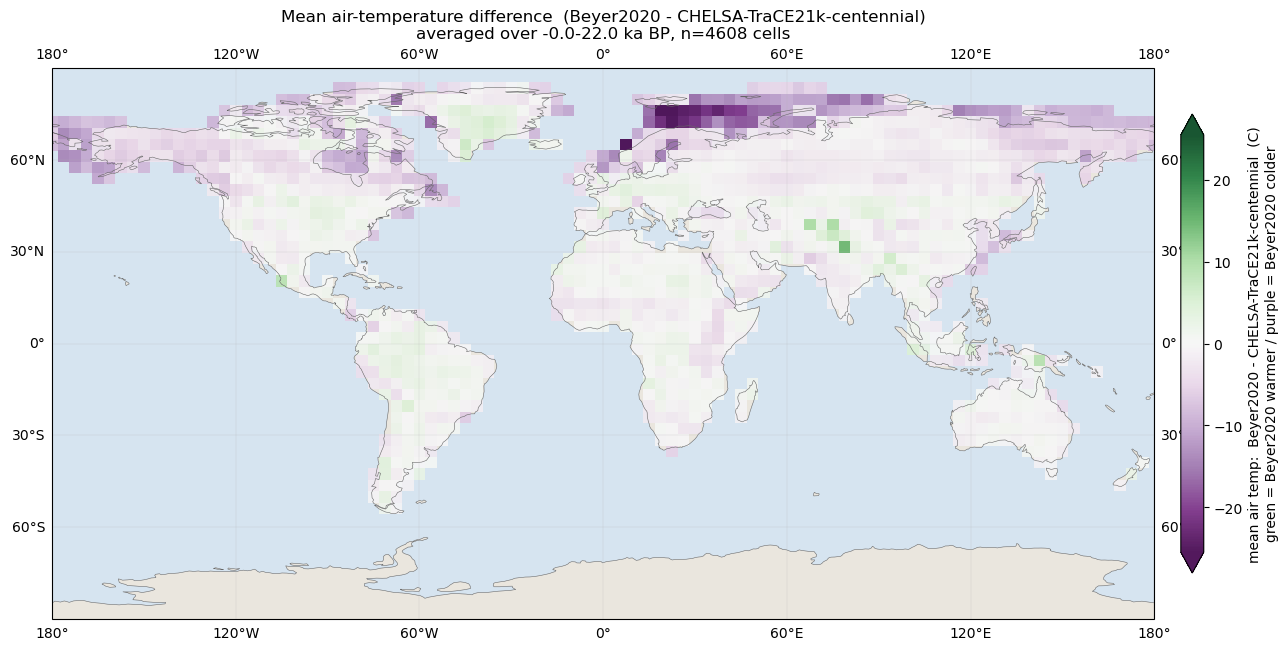
\includegraphics[width=0.72\textwidth]{diff_air_beyer2020_chelsatrace21k.png}
\caption{Mean air-temperature difference, Beyer2020 $-$ CHELSA-TraCE21k-centennial (0--22\,ka), sampled at the T31 grid and averaged over the pair's shared time window (green $=$ first archive warmer, purple $=$ colder).}
\label{fig:diff_air_beyer_chelsa}
\end{figure*}

\begin{figure*}[t]
\centering
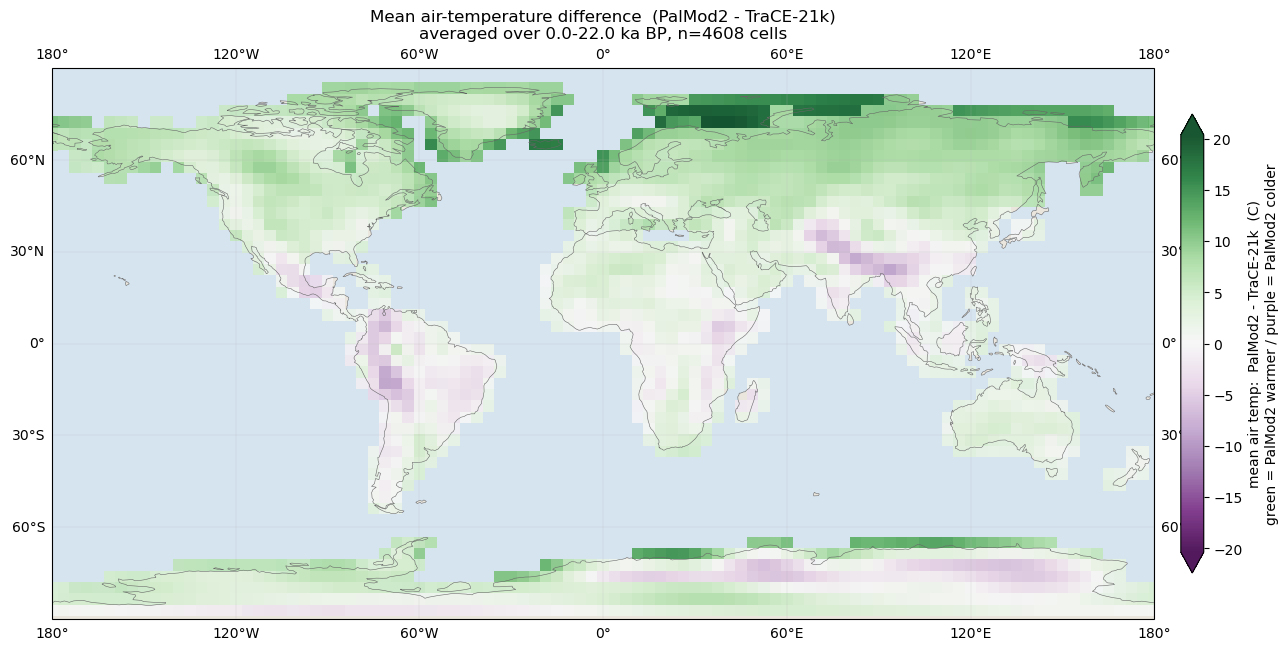
\includegraphics[width=0.72\textwidth]{diff_air_palmod2_trace21k.png}
\caption{Mean air-temperature difference, PalMod2 $-$ TraCE-21k (0--22\,ka), sampled at the T31 grid and averaged over the pair's shared time window (green $=$ first archive warmer, purple $=$ colder).}
\label{fig:diff_air_palmod2_trace21k}
\end{figure*}

\begin{figure*}[t]
\centering
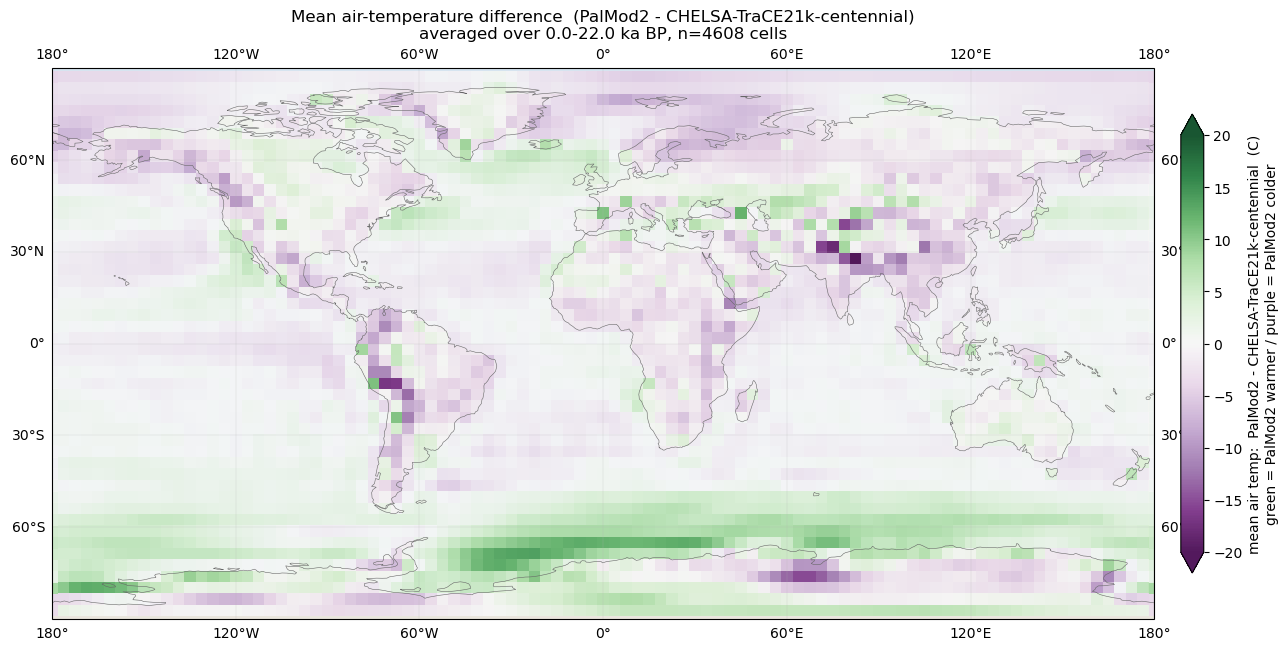
\includegraphics[width=0.72\textwidth]{diff_air_palmod2_chelsatrace21k.png}
\caption{Mean air-temperature difference, PalMod2 $-$ CHELSA-TraCE21k-centennial (0--22\,ka), sampled at the T31 grid and averaged over the pair's shared time window (green $=$ first archive warmer, purple $=$ colder).}
\label{fig:diff_air_palmod2_chelsa}
\end{figure*}

\begin{figure*}[t]
\centering
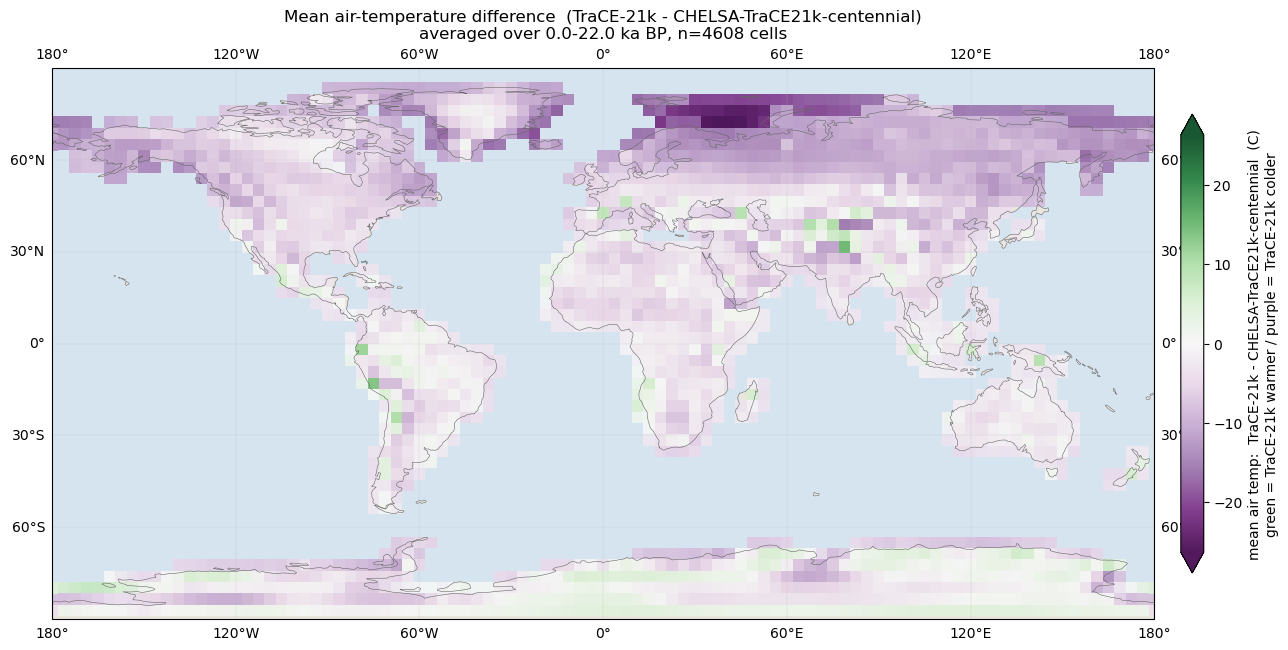
\includegraphics[width=0.72\textwidth]{diff_air_trace21k_chelsatrace21k.png}
\caption{Mean air-temperature difference, TraCE-21k $-$ CHELSA-TraCE21k-centennial (0--22\,ka), sampled at the T31 grid and averaged over the pair's shared time window (green $=$ first archive warmer, purple $=$ colder).}
\label{fig:diff_air_trace21k_chelsa}
\end{figure*}

\paragraph{Summary.} Three robust patterns emerge: (1) TraCE-21k runs systematically cool relative to all three other archives, most strongly at high northern latitudes and at the example point; (2) the two coupled GCMs differ most, in a spatially coherent high-latitude dipole, indicating structural model differences rather than noise; (3) the two observation-anchored products agree most closely, reflecting their shared present-day observational baseline.

\section{Discussion}

\subsection{Sources of inter-model difference}
The differences arise from several superimposed causes that the comparison cannot fully disentangle: (i) \emph{model physics and forcing}, since CCSM3 and MPI-ESM1.2-CR are independent models with different components, resolutions and deglacial forcing, so their large coherent high-latitude differences are genuine; (ii) \emph{downscaling and bias correction}, since Beyer2020 and CHELSA-TraCE21k-centennial are anchored to present-day observations, which pulls their late-Holocene values toward a common baseline and explains why they agree best, while the raw GCMs can deviate strongly, especially over ice-marginal high latitudes; (iii) \emph{variable definition}, since a model 2\,m diagnostic, a downscaled monthly mean and the mean of downscaled daily extremes are close but not the same quantity; (iv) \emph{spatial-scale mismatch}, since a $\sim$3.7\dg{} cell averages a region that may mix land and ocean, whereas a $\sim$1\,km pixel resolves one landscape; and (v) \emph{temporal resolution}, since annual to millennial sampling exposes very different amounts of variability.

\subsection{Limitations and caveats}\label{sec:caveats}
\textbf{Nearest-neighbour sampling.} Both the point extraction and the heatmaps use nearest-neighbour selection with no interpolation or area weighting; in the heatmaps the high-resolution archives are sub-sampled at coarse cell centres rather than averaged into them, so the maps compare representative point samples, not true area means. Conservative (area-mean) regridding would be more rigorous but far more expensive at $\sim$1\,km. \textbf{Terrestrial vs global coverage.} Beyer2020 and CHELSA-TraCE21k-centennial are land-only (Beyer2020 also excludes latitudes south of $\sim$60\dg\,S); their ocean cells are blank, so any ocean signal in a pair involving them is absent by construction. \textbf{Single example point.} The time-series results characterise one mid-latitude continental location and should not be generalised; the tool is designed to be re-run anywhere. \textbf{Source-file metadata quirk.} In the published Beyer2020 NetCDF the \tabbr{units} attributes of the two horizontal coordinates are transposed (longitude is labelled \tabbr{degrees\_north} and latitude \tabbr{degrees\_east}). This is a defect in the upstream file, not in the analysis: the tool identifies axes by name, not by their unit string, so results are unaffected.\footnote{Visible in the per-dataset inspection output (\tabbr{dataset\_info.txt}, Beyer2020 block).}

\subsection{What the comparison shows}
The exercise demonstrates both that these archives are hard to compare, since every dimension (variable, time, space, unit) requires explicit harmonisation before any number can be placed next to another, and that, once harmonised, the comparison is informative: it isolates a reproducible cool tendency in TraCE-21k, the strong structural disagreement between the two coupled GCMs at high latitudes, and the close agreement of the two observation-anchored products. These are exactly the systematic signals that flag where archives diverge and where modelling effort might be focused.

\section{Future work}
Several extensions would sharpen the analysis.

\emph{Aggregated multi-point analysis.} The extraction already accepts an arbitrary set of coordinates (Section~\ref{sec:extraction}), but the results are currently only inspected one location at a time: each point yields its own time-series overlay and coverage summary, and nothing reduces the set to a statistic. Aggregating instead of plotting, for example the mean and spread of the pairwise offsets across many points or across a whole grid, would replace the present single-point anecdote with a quantitative statement about how far the archives differ, and would close the gap between the point view and the global heatmaps, which are at present two separate products rather than two resolutions of one analysis.

\emph{Stratified analysis.} Once many points are available, the differences could be correlated with latitude band, climate zone, land versus ocean, distance to the former ice margins and elevation, moving from where the archives differ to why they differ.

\emph{Area-weighted regridding.} Conservative regridding would replace the nearest-neighbour sampling in the heatmaps, so that the high-resolution archives enter the comparison as true area means over each coarse cell rather than as one representative pixel per cell. This would remove the scale artefact identified in Section~\ref{sec:caveats}, at a considerably higher computational cost for the $\sim$1\,km archive.

\emph{Uncertainty.} The within-window temporal variability of each archive could be carried alongside the means and displayed with them, so that an apparent offset can be judged against each archive's own variability rather than taken at face value.

\emph{Further variables.} The comparison could be extended beyond
temperature to precipitation, and to the bioclimatic and vegetation fields available in Beyer2020.

\section{Conclusion}
Four heterogeneous paleoclimate temperature archives spanning the last glacial cycle were downloaded, pre-processed and harmonised onto a common \kaBP{} time axis, a common unit (\degC) and a common spatial framework, and then compared both at a point and globally. The principal difficulty is the harmonisation rather than the comparison: each archive uses a different time origin and sign convention, a different grid and longitude convention, a different temperature variable, and temporal and spatial resolutions differing by three orders of magnitude. A single time-conversion function, name-based axis detection, automatic longitude handling and unit conversion make the four directly comparable. Once harmonised, the archives agree on the first-order deglacial signal, a cold LGM followed by warming into the Holocene, but disagree on absolute temperature by several degrees, and the disagreements are neither random nor uniform: TraCE-21k is systematically cool, the two coupled GCMs diverge most strongly and coherently at high northern latitudes, and the two observation-anchored downscaling products agree most closely. The comparison cannot adjudicate which archive is correct, but it pinpoints where and by how much they differ, which is precisely the diagnostic value of inter-model comparison and a useful pointer toward where the underlying models or reconstructions most warrant scrutiny.

%-------------------------------------------------------------
{
	\begin{spacing}{1.17}
		\normalsize
		\bibliography{Bib}
	\end{spacing}
}

\end{document}